\begin{appendix} 
\section{Galaxy properties for the KiDS-1000 sources and the BOSS and 2dFLenS lenses.}
\label{app:properties}

This Appendix tabulates the properties of the KiDS-1000 tomographic source samples, along with the properties of the BOSS and 2dFLenS lens samples, in Table~\ref{tab:datatab}.   We list the spectroscopic redshift, $z_{\rm min} < z_{\rm s} \leq z_{\rm max}$, selection for the lenses, and the photometric redshift, $z_{\rm min} < z_{\rm B} \leq z_{\rm max}$, selection for the sources, along with the mean redshift of each sample.  For the source sample, the true redshift distributions are estimated using the SOM methodology from \citet{wright/etal:2020}.     The shear calibration correction $m$, which can also be refereed to in the literature as the responsivity, $R = 1+m$, is listed for each source bin \citep{kannawadi/etal:2019}.  The effective number density of lenses and sources, per square arcmin,  defines the number of galaxies per square arcmin in the case of unit weights and, for the sources, unit responsivity \citep[see equations C.11 and C.13 in][]{joachimi/etal:inprep}.  We also list the  effective ellipticity dispersion $\sigma_{\epsilon,i}$, per ellipticity component, $i$, for each the weighted and calibrated source galaxy samples \citep[equation C.8 in][]{joachimi/etal:inprep}.

\begin{table}
\caption{Blind A: Galaxy properties for the BOSS and 2dFLenS lens (\lq L\rq) samples and the KiDS-1000 source (\lq S\rq) samples.}              % title of Table
\label{tab:datatab}      % is used to refer this table in the text
\centering                                      % used for centering table
\begin{tabular}{lcccccr}          % centered columns
\hline\hline                        % inserts double horizontal lines
ID & $z_{\rm min}$ &  $z_{\rm max}$& mean $z$ & $n_{\rm eff}$ & $\sigma_{\epsilon,i}$ & \multicolumn{1}{c}{$m$}\\    % table heading
\hline
\multicolumn{6}{l}{\bf KiDS-1000:}\\  
S1 & 0.1 & 0.3 & 0.26 & 0.61 &  0.27 & $-0.009\pm0.019$\\
S2 & 0.3 & 0.5 & 0.40 & 1.17 &  0.26 & $-0.011\pm0.020$\\
S3 & 0.5 & 0.7 & 0.56 & 1.83 &  0.28 & $-0.015\pm0.017$\\
S4 & 0.7 & 0.9 & 0.79 & 1.23 &  0.26 & $0.002\pm0.012$\\
S5 & 0.9 & 1.2 & 0.98 & 1.28 &  0.28 & $0.007\pm0.010$\\
\hline      
\multicolumn{6}{l}{\bf BOSS:}\\                             % inserts single horizontal line
L1 & 0.2 & 0.5 & 0.38 & $0.014$ & -  & \multicolumn{1}{c}{-}\\
L2 & 0.5 & 0.75 & 0.61 & $0.016$ & -  & \multicolumn{1}{c}{-}\\
\hline      
\multicolumn{6}{l}{\bf 2dFLenS:}\\                                % inserts single horizontal line
L1 & 0.2 & 0.5 & 0.36 & $0.006$ & - & \multicolumn{1}{c}{-}\\
L2 & 0.5 & 0.75 & 0.60 & $0.006$ & - & \multicolumn{1}{c}{-}\\
\hline
\end{tabular}
\end{table}

%\begin{table}
%\caption{Blind B: Galaxy properties for the BOSS and 2dFLenS lens (\lq L\rq) samples and the KiDS-1000 source (\lq S\rq) samples.}              % title of Table
%\label{tab:datatab_BlindB}      % is used to refer this table in the text
%\centering                                      % used for centering table
%\begin{tabular}{lcccccr}          % centered columns
%\hline\hline                        % inserts double horizontal lines
%ID & $z_{\rm min}$ &  $z_{\rm max}$& mean $z$ & $n_{\rm eff}$ & $\sigma_{\epsilon,i}$ & \multicolumn{1}{c}{$m$}\\    % table heading
%\hline      
%\multicolumn{6}{l}{\bf KiDS-1000:}\\  
%S1 & 0.1 & 0.3 & 0.26 & 0.57 &  0.27 & $-0.009\pm0.019$\\
%S2 & 0.3 & 0.5 & 0.40 & 1.16 &  0.26 & $-0.011\pm0.020$\\
%S3 & 0.5 & 0.7 & 0.56 & 1.87 &  0.27 & $-0.015\pm0.017$\\
%S4 & 0.7 & 0.9 & 0.79 & 1.31 &  0.25 & $0.002\pm0.012$\\
%S5 & 0.9 & 1.2 & 0.99 & 1.39 &  0.26 & $0.007\pm0.010$\\
%\hline
%\multicolumn{6}{l}{\bf BOSS:}\\                             % inserts single horizontal line
%L1 & 0.2 & 0.5 & 0.38 & $0.014$ & -  & \multicolumn{1}{c}{-}\\
%L2 & 0.5 & 0.75 & 0.61 & $0.016$ & -  & \multicolumn{1}{c}{-}\\
%\hline      
%\multicolumn{6}{l}{\bf 2dFLenS:}\\                                % inserts single horizontal line
%L1 & 0.2 & 0.5 & 0.36 & $0.006$ & - & \multicolumn{1}{c}{-}\\
%L2 & 0.5 & 0.75 & 0.60 & $0.006$ & - & \multicolumn{1}{c}{-}\\
%\hline
%\end{tabular}
%\end{table}

%\begin{table}
%\caption{Blind C: Galaxy properties for the BOSS and 2dFLenS lens (\lq L\rq) samples and the KiDS-1000 source (\lq S\rq) samples.}              % title of Table
%\label{tab:datatab_BlindC}      % is used to refer this table in the text
%\centering                                      % used for centering table
%\begin{tabular}{lcccccr}          % centered columns
%\hline\hline                        % inserts double horizontal lines
%ID & $z_{\rm min}$ &  $z_{\rm max}$& mean $z$ & $n_{\rm eff}$ & $\sigma_{\epsilon,i}$ & \multicolumn{1}{c}{$m$}\\    % table heading
%\hline
%\multicolumn{6}{l}{\bf KiDS-1000:}\\  
%S1 & 0.1 & 0.3 & 0.26 & 0.57 &  0.27 & $-0.009\pm0.019$\\
%S2 & 0.3 & 0.5 & 0.40 & 1.15 &  0.26 & $-0.011\pm0.020$\\
%S3 & 0.5 & 0.7 & 0.56 & 1.84 &  0.27 & $-0.015\pm0.017$\\
%S4 & 0.7 & 0.9 & 0.79 & 1.28 &  0.26 & $0.002\pm0.012$\\
%S5 & 0.9 & 1.2 & 0.98 & 1.35 &  0.27 & $0.007\pm0.010$\\
%\hline      
%\multicolumn{6}{l}{\bf BOSS:}\\                             % inserts single horizontal line
%L1 & 0.2 & 0.5 & 0.38 & $0.014$ & -  & \multicolumn{1}{c}{-}\\
%L2 & 0.5 & 0.75 & 0.61 & $0.016$ & -  & \multicolumn{1}{c}{-}\\
%\hline      
%\multicolumn{6}{l}{\bf 2dFLenS:}\\                                % inserts single horizontal line
%L1 & 0.2 & 0.5 & 0.36 & $0.006$ & - & \multicolumn{1}{c}{-}\\
%L2 & 0.5 & 0.75 & 0.60 & $0.006$ & - & \multicolumn{1}{c}{-}\\
%\hline
%\end{tabular}
%\end{table}




\section{Parameter priors}
\label{app:priors}
This Appendix tabulates the adopted KiDS-1000 priors and sampling parameters in Table~\ref{tab:priors}.   The uniform prior on the Hubble constant, $h$, reflects distance-ladder $\pm 5 \sigma$ constraints from \citet{riess/etal:2016}, which encompasses the value of $h$ favoured by \citet{planck/etal:2018}.  The uniform prior on the CDM density, $\omega_{\rm c}$, reflects Supernova Type Ia $\pm 5 \sigma$ constraints on $\Omega_{\rm m}$ from \citet{scolnic/etal:2018} combined with the extreme values of $h$ as allowed by our $h$-prior.   The uniform prior on the baryon density, $\omega_{\rm b}$, reflects big bang nucleosynthesis $\pm 5 \sigma$ constraints from \citet{olive/etal:2014}.   As discussed in Section~\ref{sec:KCAP} we choose to sample with an uninformative uniform prior on $S_8$ to avoid implicit informative priors from a uniform prior on the primordial power spectrum amplitude $A_{\rm s}$.    We choose to impose a hard prior on the properties of neutrinos, assuming the normal hierarchy at the minimum sum of masses, $\Sigma m_\nu = 0.06$ eV, following \citet{planck/etal:2018}.  We consider extended models, including variations on neutrino mass in \citet{troester/etal:inprep}.

\begin{table}
\caption{KiDS-1000 sampling parameters and priors.}              % title of Table
\label{tab:priors}      % is used to refer this table in the text
\centering                                      % used for centering table
\begin{tabular}{lll}          % centered columns (4 columns)
\hline\hline                        % inserts double horizontal lines
Parameter & Symbol & Prior \\    % table heading
\hline                                   % inserts single horizontal line
Hubble constant & $h$ & $\bb{0.64,\,0.82}$ \\
CDM density & $\omega_{\rm c}$ & $\bb{0.051,\,0.255}$ \\
Baryon density & $\omega_{\rm b}$ & $\bb{0.019,\,0.026}$ \\
Density fluctuation amp. & $S_8$ & $\bb{0.1,\,1.3}$ \\
Scalar spectral index & $n_{\rm s}$ & $\bb{0.84,\,1.1}$ \\
\hline
Linear galaxy bias & $b_1 \;[2]$ & $\bb{0.5,\,9}$ \\
Quadratic galaxy bias & $b_2 \;[2]$ & $\bb{-0.6,\,4}$ \\
Non-local galaxy bias & ${\gamma_3^-} \;[2]$ & $\bb{-3,\,3}$ \\
Virial velocity parameter & $a_{\rm vir} \;[2]$ & $\bb{0,\,12}$ \\
Intrinsic alignment amp. & $A_{\rm IA}$ & $\bb{-6,\,6}$ \\
Baryon feedback amp. & $A_{\rm baryon}$ & $\bb{2,\,3.13}$ \\
\hline
Redshift offsets & ${\bf \delta_z}$ & ${\cal N}(\vek{\mu};\vek{C}_{\delta z})$ \\
\hline
\end{tabular}
\tablefoot{Primary cosmological parameters for the flat $\Lambda$CDM model are listed in the first section. The second section lists astrophysical nuisance parameters to model galaxy bias (with independent parameters for each of the two BOSS redshift bins as indicated with the bracket $[2]$), intrinsic galaxy alignments, and baryon feedback.  Observational redshift nuisance parameters are listed in the final section. Prior values in square brackets are the limits of the adopted uniform top-hat priors.  ${\cal N}(\mu;C)$ corresponds to a five dimensional multivariate Gaussian prior with mean $\vek{\mu}$ and covariance $\vek{C}_{\delta z}$.}
\end{table}

The uniform prior on the scalar spectral index, $n_{\rm s}$, reflects a restriction in our likelihood implementation, where the \citet{sanchez/etal:2017} galaxy clustering likelihood becomes prohibitively slow for $n_{\rm s}>1.1$.  With the upper limit of the top-hat prior fixed by this computational limitation, we choose to symmetrise the prior around the theoretical expectation of $n_{\rm s}=0.97$.     In Fig.~\ref{fig:ns-prior} we demonstrate the impact of this informative prior on the BOSS-only galaxy clustering constraints, highlighting how informative this choice of prior is.   We argue that adopting an informative prior is justified however, given our theoretical prior knowledge, and the potential for the BOSS-preference for low $n_{\rm s}$ to arise from systematic errors \citep{ross/etal:2017}.   

\begin{figure}
	\begin{center}
		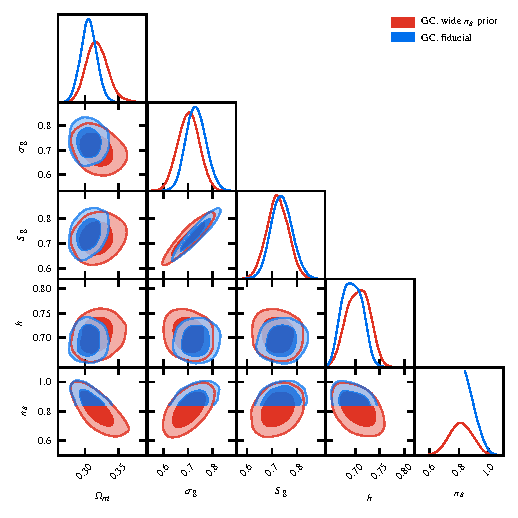
\includegraphics[width=\columnwidth]{Parameter_Plots/systematics/GC_ns_prior}
		\caption{The impact of the $n_{\rm s}$ prior: Comparing marginalised posterior distributions for the BOSS galaxy clustering analysis for our fiducial analysis (blue) with the constraints when adopting an uninformative prior on $n_{\rm s}$.   Opening the parameter space to arguably unphysical values of $n_{\rm s}$ favours lower values for $S_8$ and results in weaker constraints on $\Omega_{\rm m}$.}
		\label{fig:ns-prior}
	\end{center}
\end{figure}

Turning to astrophysical priors, the galaxy bias parameter top-hat priors, $b_1$, $b_2$,  $\gamma_3^-$, and $a_{\rm vir}$ match those adopted in \citet{sanchez/etal:2017}, with independent sets of parameters for each of the two BOSS redshift slices.   Wide uniform priors for the intrinsic alignment parameter $A_{\rm IA}$ are chosen to be uninformative.    Uniform priors on the baryon feedback parameter $A_{\rm baryon}$ are chosen such that the resulting \citet{mead/etal:2015} model of the non-linear matter power spectrum encompasses both the most aggressive feedback model from the \citet{vandaalen/etal:2011} suite of hydrodynamical simulations, along with the dark matter-only case.

There are five additional correlated nuisance parameters, $\delta^i_z$, that model uncertainty in the mean of the source redshift distributions.  We adopt a multivariate Gaussian prior for the vector $\vek{\delta}_z$ with a mean $\vek{\mu} = (0.0001,0.0021,0.0129,0.0110,-0.0060)$, and a co-variance, $C_{\delta z}$, as calibrated using mock galaxy catalogues in \citet{wright/etal:2020}.   The diagonal terms of $\vek{C}_{\delta z}$ are typically at the level of $\sim(0.01)^2$, with correlations between the different redshift bins, i.e the ratio of the off-diagonal to diagonal terms,  ranging from zero to $\sim 0.3$ \citep[see section 3.3 of][for details]{joachimi/etal:inprep}.


\section{Parameter constraints}
\label{app:parameter-constraints}
This Appendix tabulates the best-fit (MAP) and marginalised constraints on the flat $\Lambda$CDM cosmological parameters, in Table~\ref{tab:fullparams}, for the different combinations of the three large-scale structure probes considered in this work.   For constraints from KiDS-1000 cosmic shear alone, we refer the reader to \citet{asgari/etal:inprep}.
\begin{landscape}
\begin{table}
\begin{center}
\caption{Parameter constraints for the probe combinations considered in this work. \TT{EE has been left out for spacing reasons as it will be duplicated in Asgari et al.}. 
For each probe, the first column lists the MAP value with the PJ-HPDI. 
If the PJ-HPDI could not be robustly determined, no uncertainty estimate is provided. 
Probes for which no dedicated best-fit optimisation was run have their best-fit values indicated by `$\approx$'.
The second column for each probe lists the maximum of the marginal posterior, together with the marginal HPDI. 
Parameter for which the marginal probability at either prior edge exceeds 20\% of the peak probability are deemed unconstrained and are denoted by a dash. 
Finally, parameters that are not sampled are left blank.
\label{tab:fullparams}}
\begin{tabular}{lllllll}
    \toprule
    Parameter    & 3x2pt & 3x2pt& GC & GC& CS+GGL & CS+GGL \\ 
             & (best-fit) & (marginal)& (best-fit) & (marginal)& (best-fit) & (marginal) \\ 

    \midrule
$S_8     $& $0.791^{+0.02}_{-0.012}$ & $0.794^{+0.014}_{-0.018}$& $\approx 0.751^{+0.06}_{-0.04}$ & $0.735^{+0.045}_{-0.042}$& $0.793^{+0.037}_{-0.0098}$ & $0.802^{+0.016}_{-0.026}$\\
$h^2\Omega_c$& $0.133$ & $0.126^{+0.0097}_{-0.011}$& $\approx 0.127^{+0.0086}_{-0.011}$ & $0.125^{+0.0095}_{-0.01}$& $0.0545$ & --\\
$h^2\Omega_b$& $0.0248$ & --& $\approx 0.0225$ & --& $0.025$ & --\\
$h       $& $0.718$ & $0.685^{+0.029}_{-0.016}$& $\approx 0.696$ & $0.691^{+0.025}_{-0.02}$& $0.654$ & --\\
$n_s     $& $0.882$ & --& $\approx 0.85$ & --& $0.894$ & --\\
\midrule
$A_{\rm baryon}$& $3.13^{+0.0037}_{-0.47}$ & --& $$ & & $3.08$ & --\\
$A_{\rm IA}$& $1.08^{+0.25}_{-0.3}$ & $1.05^{+0.28}_{-0.28}$& $$ & & $0.958^{+0.25}_{-0.25}$ & $0.959^{+0.27}_{-0.25}$\\
$\delta \bar{z_1}$& $2.22^{+11}_{-10}\times 10^{-3}$ & $2.59^{+10}_{-11}\times 10^{-3}$& $$ & & $6.17^{+1.3e+02}_{-74}\times 10^{-4}$ & $2.35^{+7.9}_{-12}\times 10^{-3}$\\
$\delta \bar{z_2}$& $9.65^{+13}_{-7.3}\times 10^{-3}$ & $8.68^{+11}_{-9}\times 10^{-3}$& $$ & & $0.0108^{+0.013}_{-0.0079}$ & $6.47^{+12}_{-7.3}\times 10^{-3}$\\
$\delta \bar{z_3}$& $-0.0237^{+0.011}_{-0.0093}$ & $-0.0203^{+0.0092}_{-0.011}$& $$ & & $-0.0207^{+0.0068}_{-0.011}$ & $-0.0224^{+0.01}_{-0.0078}$\\
$\delta \bar{z_4}$& $-0.0146^{+0.0087}_{-0.0071}$ & $-0.0137^{+0.0081}_{-0.0079}$& $$ & & $-0.0145^{+0.0058}_{-0.01}$ & $-0.0127^{+0.007}_{-0.008}$\\
$\delta \bar{z_5}$& $5.27^{+11}_{-7}\times 10^{-3}$ & $5.95^{+9.9}_{-8.6}\times 10^{-3}$& $$ & & $6.06^{+11}_{-6.9}\times 10^{-3}$ & $7.18^{+8.3}_{-9.6}\times 10^{-3}$\\
$b_1^{\rm lowz}$& $1.95^{+0.085}_{-0.063}$ & $1.97^{+0.071}_{-0.08}$& $\approx 2^{+0.16}_{-0.11}$ & $2.07^{+0.14}_{-0.11}$& $3.78^{+0.0025}_{-1}$ & $3.2^{+0.43}_{-0.55}$\\
$b_2^{\rm lowz}$& $0.38^{+0.58}_{-0.61}$ & $0.116^{+0.73}_{-0.46}$& $\approx 0.577^{+0.96}_{-0.85}$ & $0.491^{+1.1}_{-0.8}$& $-2.67^{+3.5}_{-0.45}$ & --\\
$\gamma_3^{\rm lowz}$& $0.714^{+0.45}_{-0.43}$ & $0.827^{+0.44}_{-0.45}$& $\approx 0.327^{+0.93}_{-0.26}$ & $0.823^{+0.53}_{-0.68}$& $7.67$ & --\\
$a_{\rm vir}^{\rm lowz}$& $4.41^{+0.58}_{-1.2}$ & $4.31^{+0.83}_{-0.94}$& $\approx 4.36^{+0.92}_{-1.3}$ & $4.6^{+0.85}_{-1.3}$& $$ & \\
$b_1^{\rm highz}$& $2.07^{+0.1}_{-0.066}$ & $2.09^{+0.098}_{-0.072}$& $\approx 2.12^{+0.19}_{-0.12}$ & $2.18^{+0.18}_{-0.088}$& $2.36^{+0.39}_{-0.51}$ & $2.24^{+0.4}_{-0.51}$\\
$b_2^{\rm highz}$& $-0.957^{+0.59}_{-0.5}$ & $-1.07^{+0.74}_{-0.4}$& $\approx -1.18^{+2.4}_{-0.42}$ & $-0.846^{+2}_{-1.1}$& $3.62^{+2.9}_{-2}$ & --\\
$\gamma_3^{\rm highz}$& $0.362^{+0.73}_{-0.68}$ & $0.653^{+0.62}_{-0.73}$& $\approx -0.364^{+1.2}_{-0.89}$ & $0.142^{+0.95}_{-0.99}$& $8^{+-0.0023}_{-4.6}$ & --\\
$a_{\rm vir}^{\rm highz}$& $1.8$ & --& $\approx 0.838^{+3.2}_{-0.84}$ & --& $$ & \\
\midrule
$\sigma_8$& $0.781^{+0.025}_{-0.019}$ & $0.778^{+0.025}_{-0.02}$& $\approx 0.739^{+0.071}_{-0.032}$ & $0.731^{+0.04}_{-0.043}$& $1^{+0.16}_{-0.24}$ & $0.821^{+0.12}_{-0.13}$\\
$\sigma_{12}$& $0.744$ & $0.759^{+0.03}_{-0.026}$& $\approx 0.719^{+0.052}_{-0.038}$ & $0.711^{+0.038}_{-0.046}$& $1.01^{+0.096}_{-0.29}$ & $0.753^{+0.14}_{-0.11}$\\
$A_s     $& $1.85\times 10^{-9}$ & $1.88^{+0.23}_{-0.18}\times 10^{-9}$& $\approx 1.75^{+0.27}_{-0.21}\times 10^{-9}$ & $1.66^{+0.23}_{-0.2}\times 10^{-9}$& $1.12\times 10^{-8}$ & --\\
$\Omega_m$& $0.307$ & $0.31^{+0.011}_{-0.015}$& $\approx 0.31^{+0.012}_{-0.013}$ & $0.304^{+0.014}_{-0.011}$& $0.187^{+0.13}_{-0.043}$ & $0.275^{+0.071}_{-0.076}$\\
$100\theta_{\rm MC}$& $1.06$ & $1.05^{+0.012}_{-0.014}$& $\approx 1.05^{+0.0084}_{-0.016}$ & $1.05^{+0.0099}_{-0.014}$& $0.932^{+0.15}_{-0.007}$ & $1.07^{+0.044}_{-0.06}$\\
    \bottomrule
\end{tabular}
\end{center}
\end{table}
\end{landscape}


\section{Sensitivity tests}
\label{app:sensitivity}
In this Appendix we present, with Fig.~\ref{fig:sensitivity_tests}, the marginalised posterior distributions for a selection of the $3\times2$pt sensitivity tests explored in Sect.~\ref{sec:results}.  These tests were all shown to recover consistent constraints on $S_8$, in Fig.~\ref{fig:S8comp}, with the exception of the linear-only galaxy bias model analysis, as expected.    Here we explore these tests in more detail.    

\begin{figure*}
	\begin{center}
		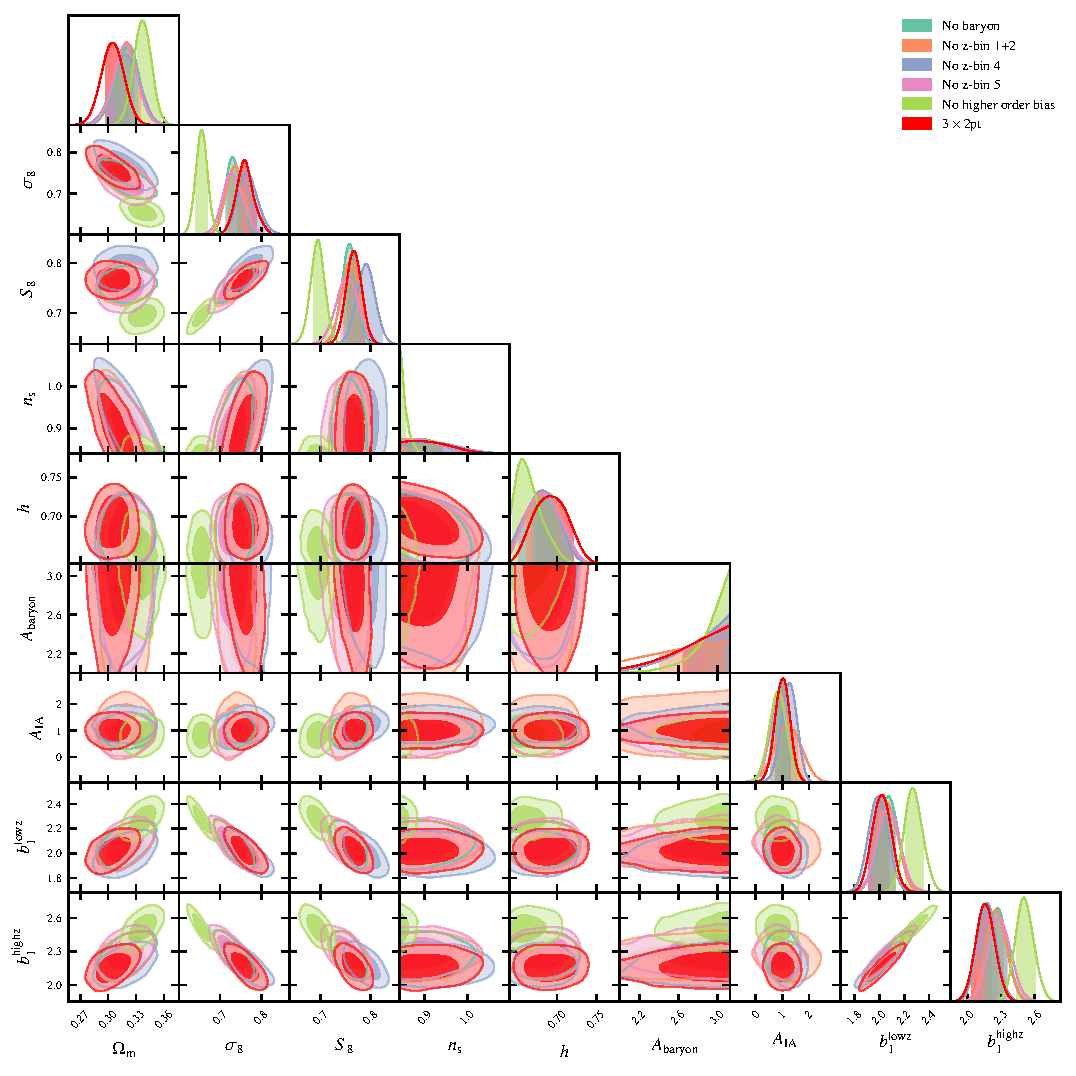
\includegraphics[width=\textwidth]{Parameter_Plots/systematics/blind_C_EE_nE_w_systematics_chains}
		\caption{Marginalised posterior distributions for the extended set of cosmological parameters shown in Fig.~\ref{fig:cosmology-params-all}, comparing the fiducial $3\times2$pt analysis (red) to a selection of our sensitivity test analyses where we ignore the impact of baryon feedback (the `No baryon' case, cyan), limit the analysis to a linear galaxy bias model (the `No higher order bias' case, green), and remove individual tomographic bins from our weak lensing observables (orange, purple and pink).  \TT{Note that the 3x2pt chain has the clustering bug fixed, hence the overall offset.}}
		\label{fig:sensitivity_tests}
	\end{center}
\end{figure*}

We compare our analysis which fully marginalises over our uncertainty in the baryon feedback parameter (red), with our `No baryon' case (cyan), where $A_{\rm baryon}=3.13$, corresponding to the non-linear matter power spectrum for a dark-matter only cosmology.   Here we find very little difference, as our $3\times2$pt analysis already favours high values of $A_{\rm baryon}$.   Our choice of scales and adoption of the band-power cosmic shear statistic for this analysis also makes us less sensitive to uncertainties in the baryon feedback parameter, compared to a standard two-point correlation function analysis \citep{asgari/etal:2020_KD}.

The removal of the two highest photometric redshift bins (blue and purple) primarily only impacts $S_8$.   These two bins carry the majority of the signal-to-noise in our analysis, and so it is not surprising that the removal of nearly half the constraining data, in each case, can result in $\sim 1 \sigma$ changes in the recovered $S_8$.   We refer the reader to \citet{asgari/etal:inprep} where we present a detailed internal consistency analysis of the cosmic shear signal, following \citet{kohlinger/etal:2019}, \citep[see also][]{efstathiou/lemos:2018},  concluding that the two highest photometric redshift bins are consistent with the full data set.   A potential $\sim 2\sigma$-level flag is, however, raised over the internal consistency of the second tomographic bin.  In our analysis where we remove the two lowest photometric redshift bins (orange), we find that these bins contribute very little to the $S_8$ constraint, and only serve to tighten the constraints on the intrinsic alignment parameter $A_{\rm IA}$.

Finally we turn to the galaxy bias test (green), where we limit the analysis to a linear galaxy bias model, $b_1$, setting all higher-order bias terms, in Eq.(\ref{eq:pgg}), to zero.   We can see that this induces a significant bias in the recovered constraints, as the amplitude of the linear galaxy bias increases in an attempt to model the enhanced power on small scales that the non-linear bias induces.   The erroneous increase in $b_1$ leads to a significant decrease in the recovered $S_8$.  This result should serve as a point of caution for $3\times2$pt analyses that adopt an effective linear bias model \citep[see also][]{asgari/etal:2020}, although we note that our analysis is particularly sensitive to the galaxy bias model given the high signal-to-noise BOSS clustering observations.


\section{Redundancy, pipeline validation and software review}
\label{app:codereview}

In this Appendix we briefly review the redundancy in the KiDS-1000 analysis, from pixels through to parameters.   Multi-band pixel processing and photometry in the optical has been carried out on the full KiDS-1000 data set using two independent pipelines, {\sc AstroWISE} and {\sc THELI} \citep{begeman/etal:2013, erben/etal:2013}.  This approach allowed us to resolve a range of different issues, primarily in the astrometric solution, for the handful of problem fields that resisted automated processing.  We adopt the {\sc AstroWISE} reduction for multi-band photometry and the {\sc THELI} $r$-band reduction for object detection and weak lensing shape measurement \citep{kuijken/etal:2019}.  We consider only one shape measurement technique, {\it lens}fit \citep{miller/etal:2013}, but this is calibrated using a series of different image simulations that vary the input galaxy properties to assess the sensitivity of the shear estimator to: the presence of blending with unresolved and undetected objects, blending due to enhanced galaxy clustering, photometric redshift selection bias, size-ellipticity correlations in the galaxy properties,  varying stellar density and the choice of galaxy profiles (smooth or realistic) \citep[see][for details]{kannawadi/etal:2019, giblin/etal:inprep}.  Our fiducial photometric redshift calibration has been compared to two additional independent calibration approaches, and has been validated on mock photometry catalogues \citep[see][for details]{wright/etal:2020, vandenbusch/etal:2020, hildebrandt/etal:inprep}.   Using a series of null-tests we have validated the resulting shear-redshift catalogues in \citet{giblin/etal:inprep}.    Our catalogue-to-observables pipeline, based on the two-point correlation function code {\sc TreeCorr} \citep{treecorr}, has been validated through an independent analysis using the alternative {\sc athena} package \citep{athena}, and through mock catalogue analysis \citep{joachimi/etal:inprep}.   Our cosmological inference code {\sc KCAP} with {\sc CAMB} \citep{lewis/etal:2000}, has been validated against the Core Cosmology Library \citep[CCL,][]{chisari/etal:2019} and through the recovery of input parameters in mock data analysis \citep{joachimi/etal:inprep}.  In \citet{asgari/etal:inprep} we also verify that we produce the same results in our cosmic-shear only analysis using a completely independent inference code based on {\sc MontePython} with {\sc CLASS} \citep{class, montepython, kohlinger/etal:2019,hildebrandt/etal:2020}.   Our analysis of BOSS follows \citet{sanchez/etal:2017}, which is in good agreement with the numerous independent parallel analyses of the same DR12 data set presented in \citet{alam/etal:2017}.

In regards to software review, we have adopted the `four-eye' approach, collaboratively building code through a git repository, with major updates reviewed through pull requests.   This approach has applied throughout the full pixels-to-parameters process, and to all types of software, both our significant tools, analysis code and, for the most part, simple paper support scripts.  On publication of this paper, our repositories will become open source for others to use and build upon, but with a caveat for users to recognise that we are not software engineers.   Adopting this style of software review for KiDS-1000 has been an extremely beneficial exercise for the team, with many lessons learnt for how to improve our software engineering skills and our approach to open source collaborative coding for future projects.     

\section{Post-unblinding analyses}
\label{app:unblinding}
This analysis was carried out `blind',  such that our final key result, our constraint on $S_8$, was unknown until all analysis choices were fixed.   Our blinding strategy creates three versions of the catalogue, where one is the truth, and the other two are modified to introduce up to a $\sim \pm 2\sigma$ deviation in the recovered value of $S_8$ \citep{kuijken/etal:2015, giblin/etal:inprep}.   In contrast to previous KiDS analyses, we set ourselves a challenge to only run our blind data analysis inference chains once, after fully developing and road-testing the pipeline using mock catalogues and data vectors \citep{joachimi/etal:inprep}.     Unexpectedly, the only chains where we failed to meet this challenge were chains that included BOSS data.   Here a bug in a naming convention in an updated {\sc CosmoSIS-CAMB} interface resulted in $\sim 0.5\sigma$ errors in the recovery of $\sigma_8$ in our initial BOSS re-analysis.

Our fiducial results, presented in Fig.~\ref{fig:cosmology-params} and tabulated in Appendix~\ref{app:parameter-constraints}, were carried out for all three blinds using a covariance matrix derived assuming a fiducial cosmology given by the best-fit parameters from \citet{troester/etal:2020}.  We reserved our iterated-covariance analysis, however, for post-unblinding, re-analysing the true data vector with an updated covariance matrix derived adopting the best-fit parameters from our initial blinded run of the true catalogue.   This iterative step changed our value for the full `$3\times2$pt' analysis $S_8$ by $X\sigma$.   Our tension-consistency analysis with the CMB constraints from Planck was also conducted after unblinding, as we were unblind to Planck throughout the process.

As we are only interested in relative shifts in the sensitivity tests presented in Fig~\ref{fig:sensitivity_tests}, these were only conducted for a single blind, and re-calculated post-unblinding for the true catalogue.  Wishing to be fully transparent in this Appendix, we note that owing to limited resources the sensitivity test was not updated during the blinded phase of the project in order to correct for the {\sc CosmoSIS-CAMB} interface error which only impacted the BOSS constraints.   We argue that this was appropriate given the nature of test and given that this error has been corrected post-unblinding.    Our cosmic shear and galaxy clustering analysis, featured in our internal consistency test in Fig.~\ref{fig:S8comp}, was also not re-processed blind after the BOSS error was corrected, as both our forecast in \citet{joachimi/etal:inprep}, and our initial analysis, confirmed that the constraints from our cosmic shear and galaxy clustering analysis were almost identical to constraints from the full `$3\times2$pt' analysis, which was correctly analysed for all three blinds.

As reported in \citet{giblin/etal:inprep}, co-author Kannawadi was unblinded early in the process to permit accurate calibration of the shear measurements in his re-analysis of KiDS-1000-like image simulations.   Co-authors Wright and Heymans also wish to record that they individually and independently had their suspicions over which blind was the truth based on the changes that the SOM gold selection made to the blinded KiDS-1000 catalogue effective number density and ellipticity dispersion, compared to the impact the SOM selection made to the KiDS-VIKING-450 catalogue analysed in \citet{wright/etal:2020b}.  These suspicions were, however, never shared with the rest of the team, nor each other.   On unblinding, these suspicions were found to be false/true(?),  and highlighted to us the challenges of catalogue-level blinding for successive data releases where little has changed in the core data reduction process.   Future KiDS blinding will therefore adopt the approach advocated by \citet{sellentin:2020}, where the covariance matrix is modified in the analysis.





\section{Plots and Tables for Blinds B and C}
%Uncomment in tex if you want to include all these extra figures

\begin{landscape}
\begin{table}
\begin{center}
\caption{Parameter constraints for blind B. }
\begin{tabular}{lllllll}
    \toprule
    Parameter    & 3x2pt & 3x2pt& GC & GC& CS+GGL & CS+GGL \\ 
             & (best-fit) & (marginal)& (best-fit) & (marginal)& (best-fit) & (marginal) \\ 

    \midrule
$S_8     $& $0.74^{+0.014}_{-0.016}$ & $0.738^{+0.017}_{-0.014}$& $\approx 0.751^{+0.06}_{-0.04}$ & $0.735^{+0.045}_{-0.042}$& $0.745^{+0.028}_{-0.039}$ & $0.723^{+0.026}_{-0.028}$\\
$h^2\Omega_c$& $0.111$ & $0.121^{+0.011}_{-0.0098}$& $\approx 0.127^{+0.0086}_{-0.011}$ & $0.125^{+0.0095}_{-0.01}$& $0.0804$ & --\\
$h^2\Omega_b$& $0.0199$ & --& $\approx 0.0225$ & --& $0.0244$ & --\\
$h       $& $0.669$ & $0.692^{+0.022}_{-0.025}$& $\approx 0.696$ & $0.691^{+0.025}_{-0.02}$& $0.663^{+0.095}_{-0.011}$ & --\\
$n_s     $& $0.935^{+0.0063}_{-0.089}$ & --& $\approx 0.85$ & --& $0.919$ & --\\
\midrule
$A_{\rm baryon}$& $3.12^{+0.0053}_{-0.48}$ & --& $$ & & $3.13$ & --\\
$A_{\rm IA}$& $1.02^{+0.31}_{-0.32}$ & $1^{+0.27}_{-0.36}$& $$ & & $0.893$ & $0.906^{+0.24}_{-0.3}$\\
$\delta \bar{z_1}$& $2.04^{+9.4}_{-12}\times 10^{-3}$ & $3.11^{+9.5}_{-12}\times 10^{-3}$& $$ & & $1.19^{+7.5}_{-12}\times 10^{-3}$ & $2.75^{+7.7}_{-12}\times 10^{-3}$\\
$\delta \bar{z_2}$& $0.0108^{+0.014}_{-0.0084}$ & $0.012^{+0.0089}_{-0.013}$& $$ & & $8.97^{+12}_{-8.2}\times 10^{-3}$ & $6.83^{+12}_{-8.7}\times 10^{-3}$\\
$\delta \bar{z_3}$& $-0.0173^{+0.01}_{-0.011}$ & $-0.0175^{+0.01}_{-0.011}$& $$ & & $-0.0188^{+0.011}_{-0.0076}$ & $-0.018^{+0.0089}_{-0.0099}$\\
$\delta \bar{z_4}$& $-0.0146^{+0.011}_{-0.0059}$ & $-0.0152^{+0.0078}_{-0.0081}$& $$ & & $-0.0143^{+0.0077}_{-0.0075}$ & $-0.0129^{+0.0076}_{-0.0078}$\\
$\delta \bar{z_5}$& $3.74^{+7.4}_{-12}\times 10^{-3}$ & $3.67^{+9.8}_{-9.2}\times 10^{-3}$& $$ & & $4.16^{+9}_{-8.9}\times 10^{-3}$ & $6.64^{+8.4}_{-9.2}\times 10^{-3}$\\
$b_1^{\rm lowz}$& $2.03^{+0.11}_{-0.047}$ & $2.1^{+0.062}_{-0.098}$& $\approx 2^{+0.16}_{-0.11}$ & $2.07^{+0.14}_{-0.11}$& $3.11$ & $3.16^{+0.66}_{-0.47}$\\
$b_2^{\rm lowz}$& $0.269^{+1.2}_{-0.33}$ & $0.301^{+0.85}_{-0.61}$& $\approx 0.577^{+0.96}_{-0.85}$ & $0.491^{+1.1}_{-0.8}$& $0.461^{+1.4}_{-3.6}$ & --\\
$\gamma_3^{\rm lowz}$& $0.621$ & $1.05^{+0.37}_{-0.69}$& $\approx 0.327^{+0.93}_{-0.26}$ & $0.823^{+0.53}_{-0.68}$& $6.72$ & --\\
$a_{\rm vir}^{\rm lowz}$& $3.97^{+1}_{-0.79}$ & $4.28^{+0.74}_{-1.1}$& $\approx 4.36^{+0.92}_{-1.3}$ & $4.6^{+0.85}_{-1.3}$& $$ & \\
$b_1^{\rm highz}$& $2.16^{+0.13}_{-0.057}$ & $2.22^{+0.088}_{-0.092}$& $\approx 2.12^{+0.19}_{-0.12}$ & $2.18^{+0.18}_{-0.088}$& $2.19^{+0.67}_{-0.54}$ & $2.26^{+0.62}_{-0.62}$\\
$b_2^{\rm highz}$& $-1.28^{+0.88}_{-0.28}$ & $-0.934^{+0.63}_{-0.57}$& $\approx -1.18^{+2.4}_{-0.42}$ & $-0.846^{+2}_{-1.1}$& $6.23^{+1.8}_{-4.3}$ & --\\
$\gamma_3^{\rm highz}$& $0.19^{+0.94}_{-0.75}$ & $0.678^{+0.7}_{-0.94}$& $\approx -0.364^{+1.2}_{-0.89}$ & $0.142^{+0.95}_{-0.99}$& $7.72^{+0.28}_{-6.4}$ & --\\
$a_{\rm vir}^{\rm highz}$& $0.831^{+1.5}_{-0.75}$ & --& $\approx 0.838^{+3.2}_{-0.84}$ & --& $$ & \\
\midrule
$\sigma_8$& $0.748^{+0.011}_{-0.03}$ & $0.736^{+0.021}_{-0.02}$& $\approx 0.739^{+0.071}_{-0.032}$ & $0.731^{+0.04}_{-0.043}$& $0.833^{+0.18}_{-0.2}$ & $0.682^{+0.099}_{-0.13}$\\
$\sigma_{12}$& $0.747$ & $0.718^{+0.025}_{-0.028}$& $\approx 0.719^{+0.052}_{-0.038}$ & $0.711^{+0.038}_{-0.046}$& $0.836^{+0.13}_{-0.25}$ & $0.619^{+0.11}_{-0.1}$\\
$A_s     $& $1.95\times 10^{-9}$ & $1.73^{+0.19}_{-0.18}\times 10^{-9}$& $\approx 1.75^{+0.27}_{-0.21}\times 10^{-9}$ & $1.66^{+0.23}_{-0.2}\times 10^{-9}$& $4.13^{+5.3}_{-3.4}\times 10^{-9}$ & --\\
$\Omega_m$& $0.293^{+0.024}_{-0.00098}$ & $0.304^{+0.01}_{-0.014}$& $\approx 0.31^{+0.012}_{-0.013}$ & $0.304^{+0.014}_{-0.011}$& $0.24^{+0.14}_{-0.069}$ & $0.316^{+0.096}_{-0.082}$\\
$100\theta_{\rm MC}$& $1.04$ & $1.05^{+0.013}_{-0.012}$& $\approx 1.05^{+0.0084}_{-0.016}$ & $1.05^{+0.0099}_{-0.014}$& $0.983^{+0.12}_{-0.035}$ & $1.1^{+0.029}_{-0.06}$\\
    \bottomrule
\end{tabular}
\end{center}
\end{table}
\end{landscape}

\begin{landscape}
\begin{table}
\begin{center}
\caption{Parameter constraints for the probe combinations considered in this work: \tttp, cosmic shear (CS) and galaxy-galaxy lensing (GGL), cosmic shear and galaxy clustering (GC), and galaxy clustering by itself. 
We refer the reader to \citet{asgari/etal:inprep} for cosmic shear-only constraints. 
For each probe, the first column lists the MAP value with the PJ-HPD CI. 
If the PJ-HPD CI could not be robustly determined, no uncertainty estimate is provided. 
The second column for each probe lists the maximum of the marginal posterior, together with the marginal HPD CI. 
Parameter for which the marginal probability at either prior edge exceeds 13\% of the peak probability are deemed unconstrained and are denoted by a dash. 
Finally, parameters that are not sampled are left blank.
\label{tab:fullparams}}
\begin{tabular}{lllllllll}
    \toprule
    Parameter    & $3\times2$pt & $3\times2$pt& GC & GC& CS+GGL & CS+GGL& CS+GC & CS+GC \\ 
             & (joint) & (marginal)& (joint) & (marginal)& (joint) & (marginal)& (joint) & (marginal) \\ 

    \midrule
$S_8     $& $0.766^{+0.02}_{-0.014}$ & $0.765^{+0.017}_{-0.016}$& $0.762^{+0.054}_{-0.05}$ & $0.743^{+0.038}_{-0.05}$& $0.774^{+0.031}_{-0.029}$ & $0.761^{+0.024}_{-0.025}$& $0.766^{+0.018}_{-0.015}$ & $0.763^{+0.016}_{-0.016}$\\ [0.3 em]
$h^2\Omega_\mathrm{c}$& $0.123$ & $0.124^{+0.0096}_{-0.011}$& $0.136^{+0.0065}_{-0.018}$ & $0.123^{+0.011}_{-0.009}$& $0.0721^{+0.089}_{-0.016}$ & $0.12^{+0.057}_{-0.034}$& $0.126^{+0.0075}_{-0.013}$ & $0.124^{+0.01}_{-0.011}$\\ [0.3 em]
$h^2\Omega_\mathrm{b}$& $0.0225$ & --& $0.0246^{+0.0012}_{-0.0037}$ & --& $0.0258$ & --& $0.0219^{+0.0022}_{-0.0022}$ & --\\ [0.3 em]
$h       $& $0.695^{+0.03}_{-0.019}$ & $0.696^{+0.02}_{-0.026}$& $0.716^{+0.02}_{-0.035}$ & $0.687^{+0.029}_{-0.018}$& $0.642^{+0.1}_{-1.2e-05}$ & --& $0.695^{+0.022}_{-0.023}$ & $0.69^{+0.026}_{-0.02}$\\ [0.3 em]
$n_\mathrm{s}$& $0.901$ & --& $0.851^{+0.06}_{-0.01}$ & --& $0.947$ & --& $0.894^{+0.05}_{-0.042}$ & --\\ [0.3 em]
\midrule
$A_{\rm bary}$& $3.13^{+1.6e-05}_{-0.47}$ & --& $$ & & $3.13$ & --& $3.13$ & --\\ [0.3 em]
$A_{\rm IA}$& $1.07^{+0.27}_{-0.31}$ & $1.01^{+0.31}_{-0.28}$& $$ & & $0.974^{+0.32}_{-0.2}$ & $0.972^{+0.25}_{-0.26}$& $0.947^{+0.44}_{-0.31}$ & $0.892^{+0.35}_{-0.36}$\\ [0.3 em]
$\delta \bar{z_1}$& $1.93^{+11}_{-10}\times 10^{-3}$ & $2.8^{+8.8}_{-12}\times 10^{-3}$& $$ & & $1.41^{+8.4}_{-11}\times 10^{-3}$ & $2.15^{+8.7}_{-11}\times 10^{-3}$& $2.02^{+7.4}_{-14}\times 10^{-3}$ & $2.45^{+9.5}_{-12}\times 10^{-3}$\\ [0.3 em]
$\delta \bar{z_2}$& $0.0101^{+0.016}_{-0.0068}$ & $9.09^{+-9.1}_{-9.1}$& $$ & & $0.0102^{+0.014}_{-0.0069}$ & $8.75^{+-8.7}_{-8.8}$& $0.0117^{+0.013}_{-0.0085}$ & $0.0121^{+0.0095}_{-0.012}$\\ [0.3 em]
$\delta \bar{z_3}$& $-0.0207^{+0.0093}_{-0.01}$ & $-0.0204^{+0.01}_{-0.0093}$& $$ & & $-0.0206^{+0.0091}_{-0.0091}$ & $-0.0199^{+0.0092}_{-0.0092}$& $-0.013^{+0.0091}_{-0.012}$ & $-0.0119^{+0.0098}_{-0.011}$\\ [0.3 em]
$\delta \bar{z_4}$& $-0.0143^{+0.0076}_{-0.008}$ & $-0.0145^{+0.0082}_{-0.0076}$& $$ & & $-0.0138^{+0.0066}_{-0.0086}$ & $-0.012^{+0.0062}_{-0.009}$& $-0.0166^{+0.0098}_{-0.0064}$ & $-0.0156^{+0.0077}_{-0.0085}$\\ [0.3 em]
$\delta \bar{z_5}$& $5.23^{+8.3}_{-10}\times 10^{-3}$ & $4.54^{+10}_{-8.7}\times 10^{-3}$& $$ & & $6.06^{+7.3}_{-10}\times 10^{-3}$ & $6.85^{+8.7}_{-8.6}\times 10^{-3}$& $6.5^{+12}_{-7.1}\times 10^{-3}$ & $6.54^{+9.4}_{-9}\times 10^{-3}$\\ [0.3 em]
$b_1^{\rm lowz}$& $2^{+0.079}_{-0.083}$ & $2.04^{+0.064}_{-0.093}$& $2.01^{+0.13}_{-0.16}$ & $2.09^{+0.11}_{-0.13}$& $3.29^{+0.3}_{-0.81}$ & $3.14^{+0.55}_{-0.55}$& $1.99^{+0.09}_{-0.07}$ & $2.02^{+0.085}_{-0.07}$\\ [0.3 em]
$b_2^{\rm lowz}$& $0.3^{+0.62}_{-0.69}$ & $0.289^{+0.71}_{-0.61}$& $0.475^{+1.1}_{-0.83}$ & $0.624^{+0.96}_{-1}$& $0.968$ & --& $0.443^{+1}_{-0.67}$ & $0.326^{+1}_{-0.67}$\\ [0.3 em]
$\gamma_{3-}^{\rm lowz}$& $0.695^{+0.48}_{-0.54}$ & $0.879^{+0.44}_{-0.52}$& $0.688^{+0.59}_{-0.57}$ & $0.752^{+0.62}_{-0.56}$& $7.87$ & --& $0.594^{+0.58}_{-0.57}$ & $0.853^{+0.53}_{-0.52}$\\ [0.3 em]
$a_{\rm vir}^{\rm lowz}$& $4.14^{+0.84}_{-0.97}$ & $4.24^{+0.86}_{-0.96}$& $4.3^{+1.1}_{-1.2}$ & $4.44^{+1.1}_{-1.2}$& $$ & & $4.28^{+1.2}_{-1}$ & $4.37^{+1.1}_{-1.1}$\\ [0.3 em]
$b_1^{\rm highz}$& $2.13^{+0.095}_{-0.091}$ & $2.17^{+0.083}_{-0.093}$& $2.14^{+0.16}_{-0.16}$ & $2.23^{+0.13}_{-0.14}$& $2.3^{+0.33}_{-0.68}$ & $2.26^{+0.48}_{-0.52}$& $2.12^{+0.1}_{-0.094}$ & $2.17^{+0.092}_{-0.084}$\\ [0.3 em]
$b_2^{\rm highz}$& $-1.15^{+0.75}_{-0.41}$ & $-1.03^{+0.72}_{-0.46}$& $-0.948^{+2.3}_{-0.75}$ & $-0.901^{+2.3}_{-1}$& $5.82^{+2}_{-3.2}$ & --& $-1.16^{+1.8}_{-0.48}$ & $-0.951^{+1.7}_{-0.85}$\\ [0.3 em]
$\gamma_{3-}^{\rm highz}$& $0.369^{+0.8}_{-0.79}$ & $0.505^{+0.9}_{-0.62}$& $-0.126^{+0.94}_{-1.1}$ & $0.452^{+0.7}_{-1.2}$& $8^{+0.00058}_{-5.4}$ & --& $-0.0141^{+0.91}_{-0.91}$ & $0.412^{+0.8}_{-0.81}$\\ [0.3 em]
$a_{\rm vir}^{\rm highz}$& $1.18^{+1.5}_{-0.97}$ & --& $1.84^{+2.4}_{-1.8}$ & --& $$ & & $1.32^{+2.7}_{-1.3}$ & --\\ [0.3 em]
\midrule
$\Omega_\mathrm{m}$& $0.305^{+0.01}_{-0.015}$ & $0.306^{+0.012}_{-0.013}$& $0.313^{+0.0097}_{-0.017}$ & $0.307^{+0.011}_{-0.015}$& $0.239^{+0.11}_{-0.076}$ & $0.29^{+0.087}_{-0.07}$& $0.306^{+0.013}_{-0.012}$ & $0.307^{+0.012}_{-0.014}$\\ [0.3 em]
$\sigma_8$& $0.76^{+0.025}_{-0.02}$ & $0.759^{+0.02}_{-0.024}$& $0.75^{+0.045}_{-0.047}$ & $0.725^{+0.048}_{-0.036}$& $0.867^{+0.2}_{-0.17}$ & $0.729^{+0.13}_{-0.098}$& $0.758^{+0.028}_{-0.018}$ & $0.758^{+0.019}_{-0.024}$\\ [0.3 em]
$\sigma_{12}$& $0.743^{+0.03}_{-0.026}$ & $0.737^{+0.029}_{-0.027}$& $0.717^{+0.058}_{-0.035}$ & $0.707^{+0.046}_{-0.04}$& $0.887^{+0.15}_{-0.23}$ & $0.72^{+0.095}_{-0.14}$& $0.734$ & $0.732^{+0.03}_{-0.024}$\\ [0.3 em]
$S_{12}  $& $0.754^{+0.021}_{-0.013}$ & $0.754^{+0.015}_{-0.018}$& $0.751^{+0.038}_{-0.054}$ & $0.728^{+0.041}_{-0.045}$& $0.77^{+0.067}_{-0.046}$ & $0.757^{+0.036}_{-0.05}$& $0.753^{+0.022}_{-0.013}$ & $0.754^{+0.014}_{-0.019}$\\ [0.3 em]
$A_\mathrm{s}$& $1.85^{+0.25}_{-0.17}\times 10^{-9}$ & $1.79^{+0.22}_{-0.18}\times 10^{-9}$& $1.7^{+0.33}_{-0.16}\times 10^{-9}$ & $1.64^{+0.27}_{-0.18}\times 10^{-9}$& $5.34^{+5.2}_{-4.3}\times 10^{-9}$ & --& $1.81^{+0.27}_{-0.15}\times 10^{-9}$ & $1.78^{+0.21}_{-0.18}\times 10^{-9}$\\ [0.3 em]
$100\theta_{\rm MC}$& $1.05$ & $1.05^{+0.011}_{-0.015}$& $1.06^{+0.0082}_{-0.019}$ & $1.05^{+0.012}_{-0.013}$& $0.96^{+0.13}_{-0.023}$ & $1.09^{+0.039}_{-0.058}$& $1.05^{+0.009}_{-0.016}$ & $1.05^{+0.012}_{-0.014}$\\ [0.3 em]
    \bottomrule
\end{tabular}


\end{center}
\end{table}
\end{landscape}



\begin{figure}
	\begin{center}
		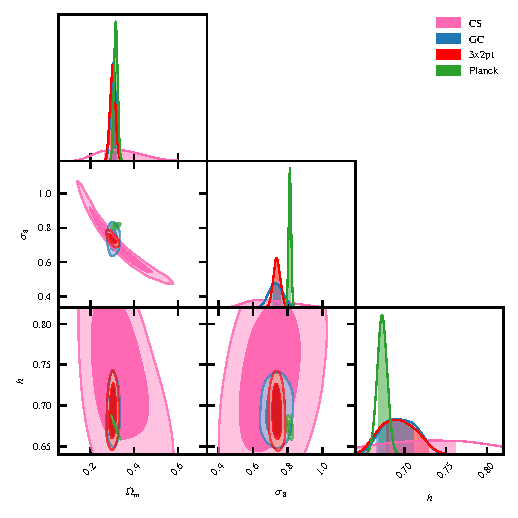
\includegraphics[width=\columnwidth]{Parameter_Plots/cosmology/omegam_sigma8_h_blind_B}
		\caption{Constraints on flat $\Lambda$CDM blind B}
		\label{fig:cosmology-params}
	\end{center}
\end{figure}

\begin{figure}
	\begin{center}
		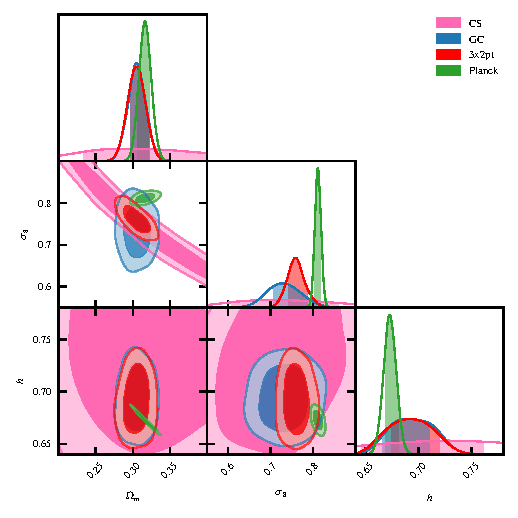
\includegraphics[width=\columnwidth]{Parameter_Plots/cosmology/omegam_sigma8_h_blind_C}
		\caption{Constraints on flat $\Lambda$CDM blind C}
		\label{fig:cosmology-params}
	\end{center}
\end{figure}


\begin{figure}
	\begin{center}
		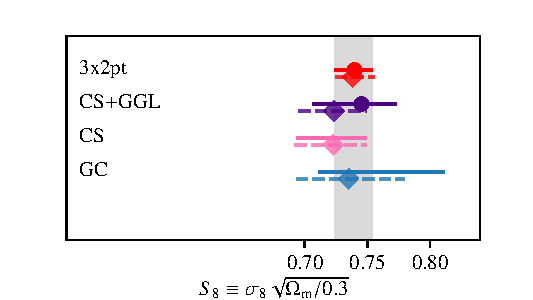
\includegraphics[width=\columnwidth]{Parameter_Plots/systematics/S8_comparison_blindB}
		\caption{Constraints on $S_{8}$ blind B}
		\label{fig:S8comp}
	\end{center}
\end{figure}

\begin{figure}
	\begin{center}
		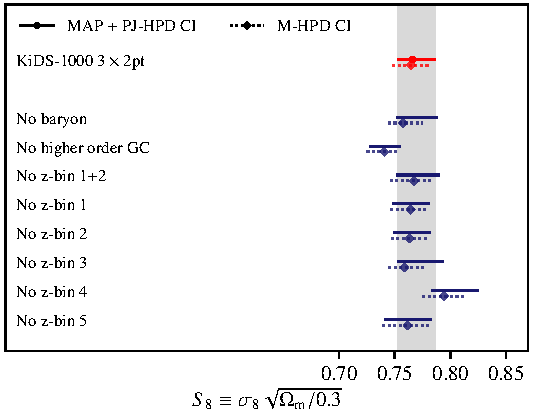
\includegraphics[width=\columnwidth]{Parameter_Plots/systematics/S8_comparison_blindC}
		\caption{Constraints on $S_{8}$ blind C}
		\label{fig:S8comp}
	\end{center}
\end{figure}


\begin{figure*}
	\begin{center}
		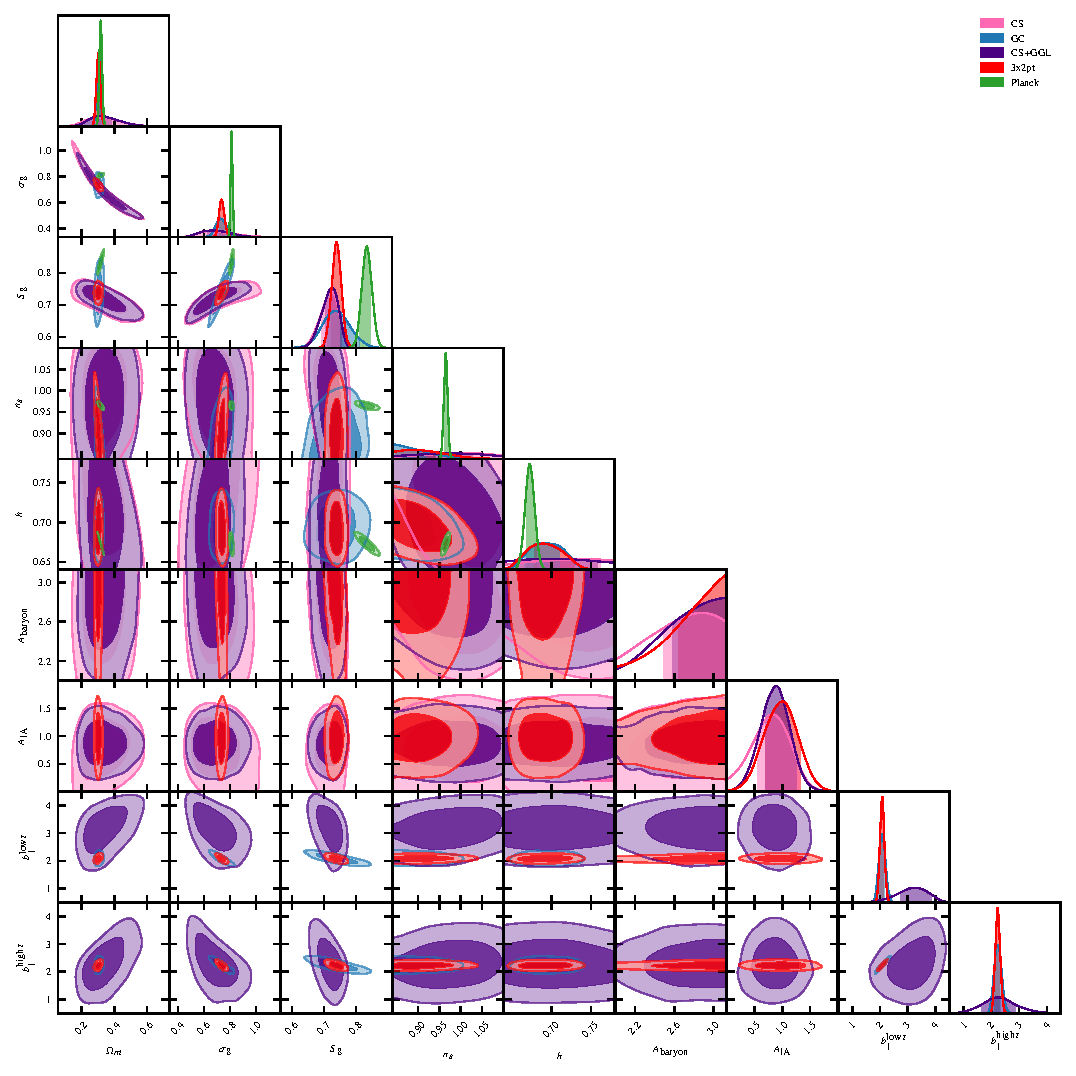
\includegraphics[width=\textwidth]{Parameter_Plots/cosmology/omegam_sigma8_s8_ns_h_a_baryon_a_ia_b1l_b1h_blind_B}
		\caption{Constraints blind B}
		\label{fig:cosmology-params-all}
	\end{center}
\end{figure*}

\begin{figure*}
	\begin{center}
		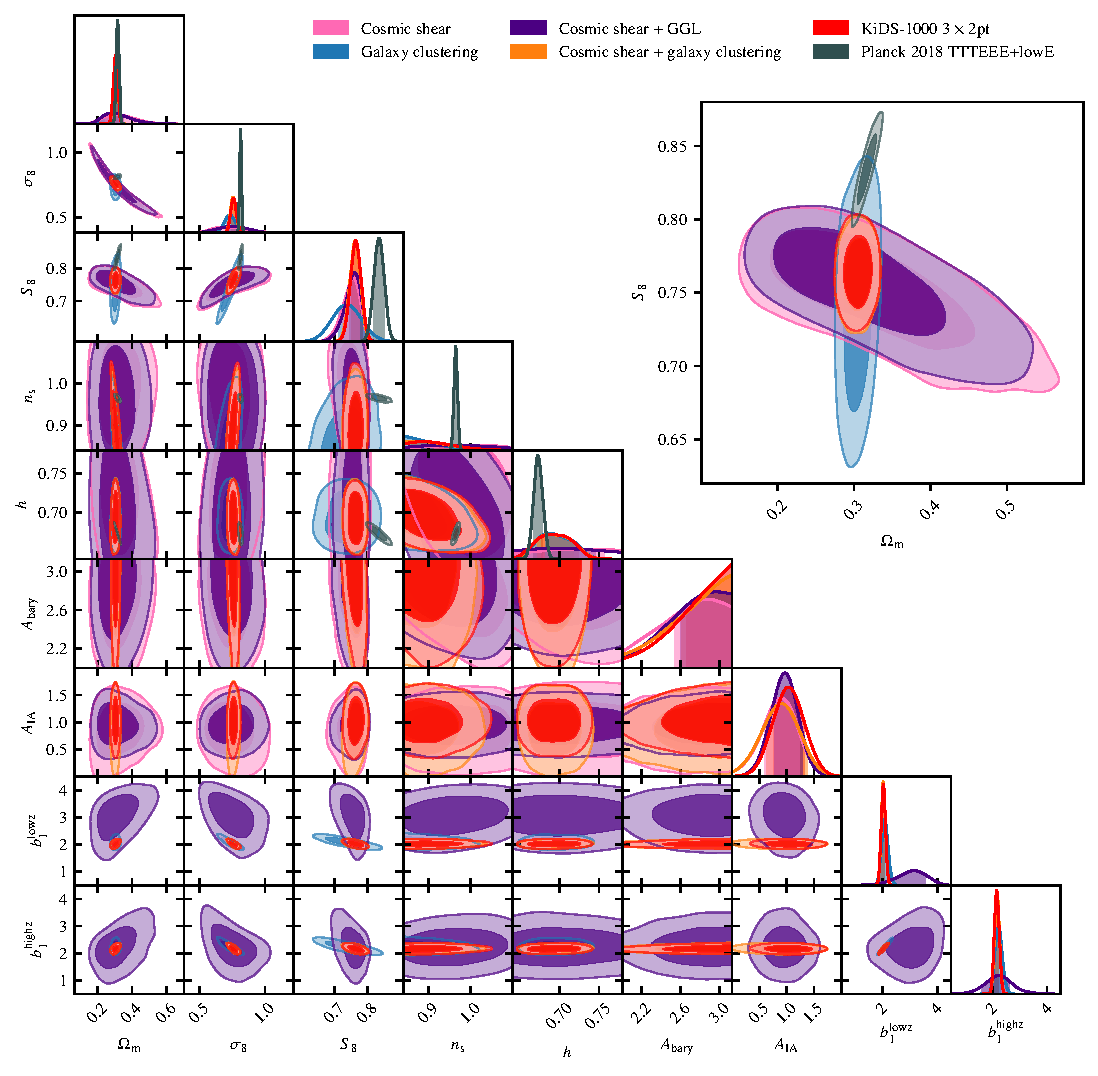
\includegraphics[width=\textwidth]{Parameter_Plots/cosmology/omegam_sigma8_s8_ns_h_a_baryon_a_ia_b1l_b1h_blind_C}
		\caption{Constraints blind C}
		\label{fig:cosmology-params-all}
	\end{center}
\end{figure*}

\begin{table}
	\begin{center}
		\caption{Goodness of fit for blind B}
		\label{tab:goodness-of-fit}
\begin{tabular}{lrcl}
    \toprule
    Probe             & $\chi^2$       & DoF       & $p$-value   \\
    \midrule
	EE               & $< 151.3$ & $120-4.5$ & 0.014 \\
	w                & $< 176.0$ & $168-13$ & 0.119 \\
	EE+nE            & $< 176.1$ & $142-18$ & 0.001 \\
	EE+w             & $< 328.0$ & $288-20$ & 0.007 \\
	EE+nE+w          & $351.3$ & $310-20$ & 0.008 \\
	
    \bottomrule
\end{tabular}
	\end{center}
\end{table}

\begin{table}
	\begin{center}
		\caption{Goodness of fit for blind C}
		\label{tab:goodness-of-fit}
\begin{tabular}{lrcl}
    \toprule
    Probe             & $\chi^2$       & DoF       & $p$-value   \\
    \midrule
	EE               & $< 150.8$ & $120-4.5$ & 0.015 \\
	w                & $< 176.0$ & $168-13$ & 0.119 \\
	EE+nE            & $< 178.5$ & $142-18$ & 0.001 \\
	EE+w             & $< 321.7$ & $288-20$ & 0.014 \\
	EE+nE+w          & $356.1$ & $310-20$ & 0.005 \\

    \bottomrule
\end{tabular}
	\end{center}
\end{table}



\end{appendix}